\documentclass[12pt,letterpaper]{article}

\usepackage[spanish]{babel}
\usepackage[utf8]{inputenc}
\usepackage[T1]{fontenc}
\usepackage{amsmath,amssymb}
\usepackage[margin=2.4cm]{geometry}
\usepackage{graphicx}
\usepackage{float}
\usepackage{enumitem}
\usepackage{parskip}
\usepackage{booktabs}

\setlength{\parindent}{0pt}
\setlength{\parskip}{5pt}

% ────────────────────────────────────────────
\begin{document}

\begin{center}
  {\LARGE\bfseries Tarea 3}\\[6pt]
  {\large UEA: Modelación Matemática I}\\[4pt]
  {\large Autor: Alejandro Cruz López}
\end{center}

\bigskip
\noindent\rule{\textwidth}{0.5pt}
\bigskip

% ============================================================
\noindent\textbf{Ejercicio 1.} Considérese el siguiente sistema de ecuaciones diferenciales
\[
  x' = 2x - x^2 + 2xy, \qquad y' = 2y - y^2 + 2xy.
\]

\noindent\textbf{a) Interpretación biológica.}

Factorizando:
\[
  x' = x(2 - x + 2y), \qquad y' = y(2 - y + 2x).
\]
Las tasas de crecimiento per cápita son:
\[
  \frac{x'}{x} = 2 - x + 2y, \qquad \frac{y'}{y} = 2 - y + 2x.
\]
Los términos $2x,\,2y$ representan crecimiento intrínseco; los términos $-x^2,\,-y^2$
representan autorregulación (competencia intraespecífica); los términos $+2xy$ en ambas
ecuaciones representan interacción benéfica mutua, pues
\[
  \frac{\partial}{\partial y}\!\left(\frac{x'}{x}\right) = 2 > 0,
  \qquad
  \frac{\partial}{\partial x}\!\left(\frac{y'}{y}\right) = 2 > 0.
\]
El sistema modela dos especies con crecimiento logístico propio y una interacción \textbf{mutualista fuerte}.

\bigskip
\noindent\textbf{b) Puntos de equilibrio.}

De $x'=0$: $x=0$ o $x = 2+2y$.
De $y'=0$: $y=0$ o $y = 2+2x$.

\begin{itemize}
  \item $x=0,\,y=0 \;\to\; (0,0)$.
  \item $y=0$: $x(2-x)=0 \Rightarrow x=2 \;\to\; (2,0)$.
  \item $x=0$: $y(2-y)=0 \Rightarrow y=2 \;\to\; (0,2)$.
  \item $x=2+2y$ y $y=2+2x$: sustituyendo, $x = 2+2(2+2x) = 6+4x \Rightarrow -3x=6
    \Rightarrow x=-2,\; y=-2$.
\end{itemize}

\[
  \boxed{(0,0),\quad (2,0),\quad (0,2),\quad (-2,-2).}
\]

Solo $(0,0)$, $(2,0)$ y $(0,2)$ pertenecen al dominio biológico $\mathbb{R}_{\geq 0}^2$.
El punto $(-2,-2)$ es un equilibrio matemático sin interpretación poblacional.

\bigskip
\noindent\textbf{c) Linealización.}

\[
  DF(x,y) = \begin{pmatrix} 2-2x+2y & 2x \\ 2y & 2-2y+2x \end{pmatrix}.
\]

\begin{table}[H]
\centering
\begin{tabular}{lccc}
\toprule
Equilibrio & Jacobiana & Valores propios & Clasificación \\
\midrule
$(0,0)$ & $\begin{pmatrix}2&0\\0&2\end{pmatrix}$ & $2,\;2$ & Nodo fuente (inestable) \\[8pt]
$(2,0)$ & $\begin{pmatrix}-2&4\\0&6\end{pmatrix}$ & $-2,\;6$ & Punto silla \\[8pt]
$(0,2)$ & $\begin{pmatrix}6&0\\4&-2\end{pmatrix}$ & $6,\;-2$ & Punto silla \\[8pt]
$(-2,-2)$ & $\begin{pmatrix}2&-4\\-4&2\end{pmatrix}$ & $-2,\;6$ & Punto silla (sin sentido biológico) \\
\bottomrule
\end{tabular}
\end{table}

Para $(-2,-2)$: $(2-\lambda)^2 - 16 = 0 \Rightarrow 2-\lambda = \pm4 \Rightarrow \lambda_1=-2,\;\lambda_2=6$.

\bigskip
\noindent\textbf{d) Isoclinas nulas y signos por región.}

Las isoclinas son $x=0$, $x=2+2y$, $y=0$, $y=2+2x$. En el interior del primer cuadrante ($x,y>0$) el signo de $x'$ depende solo de $2-x+2y$ y el de $y'$ de $2-y+2x$:

\begin{table}[H]
\centering
\begin{tabular}{lcc}
\toprule
Región & $x'$ & $y'$ \\
\midrule
$x < 2+2y$ y $y < 2+2x$ (región central) & $+$ & $+$ \\
$x > 2+2y$ & $-$ & $+$ \\
$y > 2+2x$ & $+$ & $-$ \\
\bottomrule
\end{tabular}
\end{table}

No existe región del primer cuadrante con $x'<0$ y $y'<0$ simultáneamente: el sistema nunca empuja a ambas poblaciones hacia la extinción a la vez.

\bigskip
\noindent\textbf{e) Dinámica sobre los ejes.}

Sobre el eje $x$ ($y=0$): $x'=x(2-x)$, línea de fase logística con $x=2$ estable sobre el eje. Análogamente, sobre el eje $y$: $y=2$ es estable sobre el eje. Sin embargo, $(2,0)$ y $(0,2)$ son sillas en el plano completo: solo son estables si la otra especie parte exactamente en cero.

\bigskip
\noindent\textbf{f) Comportamiento interior.}

Para $x,y>0$:
\[
  (xy)' = xy(4+x+y) > 0.
\]
El producto $xy$ es estrictamente creciente. Definiendo $u=\sqrt{xy}$ y usando $x+y\geq2u$:
\[
  u' = \frac{u(4+x+y)}{2} \geq \frac{u(2u)}{2} = u^2.
\]
Las trayectorias interiores no convergen a equilibrio positivo alguno: el mutualismo cuadrático produce \textbf{crecimiento no acotado}.

\bigskip
\noindent\textbf{g) Bosquejo del retrato fase.}

\begin{figure}[H]
  \centering
  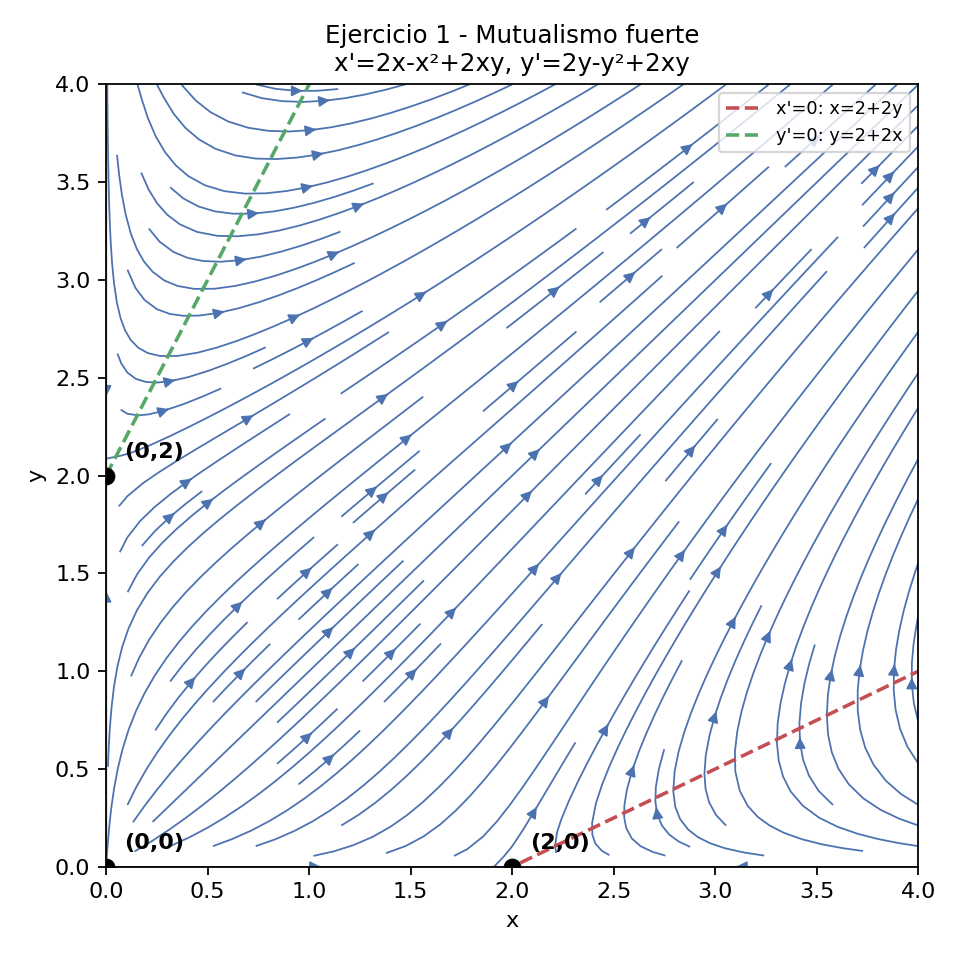
\includegraphics[width=0.72\textwidth]{figs/ejercicio1_mutualismo_fuerte.png}
  \caption{Retrato fase del sistema mutualista fuerte. Las isoclinas $x=2+2y$ (rojo) e
           $y=2+2x$ (verde) no se cortan en el primer cuadrante. Las trayectorias interiores
           se alejan hacia el noreste de forma no acotada.}
\end{figure}

\bigskip
\noindent\textbf{h) Conclusiones biológicas.}

\begin{table}[H]
\centering
\begin{tabular}{ll}
\toprule
Condición inicial & Comportamiento a largo plazo \\
\midrule
$x_0=0,\;y_0=0$ & Extinción total (inestable, no se sostiene) \\
$x_0>0,\;y_0=0$ & $\to(2,0)$: sobrevive solo $x$ \\
$x_0=0,\;y_0>0$ & $\to(0,2)$: sobrevive solo $y$ \\
$x_0>0,\;y_0>0$ & Ambas persisten, pero con crecimiento no acotado \\
\bottomrule
\end{tabular}
\end{table}

No es posible la extinción de ambas desde condiciones interiores positivas. La extinción de una sola especie solo ocurre si la otra parte exactamente en cero. La coexistencia existe en el sentido de que ambas permanecen positivas, pero no es regulada: el modelo describe un mutualismo no saturado, poco realista a tiempos largos por carecer de limitación global de recursos.

\bigskip
\noindent\rule{\textwidth}{0.3pt}
\bigskip

% ============================================================
\noindent\textbf{Ejercicio 2.} Considérese el siguiente sistema de ecuaciones diferenciales
\[
  x' = 2x - 2x^2 + xy, \qquad y' = 2y - 2y^2 + xy.
\]

\noindent\textbf{a) Interpretación biológica.}

Factorizando:
\[
  x' = x(2-2x+y), \qquad y' = y(2-2y+x).
\]
\[
  \frac{x'}{x} = 2 - 2x + y, \qquad \frac{y'}{y} = 2 - 2y + x.
\]

Los términos $-2x^2,\,-2y^2$ representan autorregulación \textbf{más fuerte} que en el Ejercicio~1
(coeficiente $2$ en lugar de $1$, mayor costo por sobrepoblación). Los términos $+xy$ mantienen
la cooperación pero con coeficiente $1$ en lugar de $2$ (beneficio más débil). Como
\[
  \frac{\partial}{\partial y}\!\left(\frac{x'}{x}\right)=1>0,
  \qquad
  \frac{\partial}{\partial x}\!\left(\frac{y'}{y}\right)=1>0,
\]
sigue siendo \textbf{mutualismo}, pero más moderado: mayor competencia interna y menor cooperación.

\bigskip
\noindent\textbf{b) Puntos de equilibrio.}

De $x'=0$: $x=0$ o $y=2x-2$.
De $y'=0$: $y=0$ o $x=2y-2$.

\begin{itemize}
  \item $x=0,\,y=0 \;\to\; (0,0)$.
  \item $y=0$: $x(2-2x)=0 \Rightarrow x=1 \;\to\; (1,0)$.
  \item $x=0$: $y(2-2y)=0 \Rightarrow y=1 \;\to\; (0,1)$.
  \item $y=2x-2$ y $x=2y-2$: sustituyendo, $x = 2(2x-2)-2 = 4x-6 \Rightarrow -3x=-6
    \Rightarrow x=2,\; y=2$.
\end{itemize}

\[
  \boxed{(0,0),\quad (1,0),\quad (0,1),\quad (2,2).}
\]

A diferencia del Ejercicio~1, los cuatro equilibrios son biológicamente válidos.

\bigskip
\noindent\textbf{c) Linealización.}

\[
  DF(x,y) = \begin{pmatrix} 2-4x+y & x \\ y & 2-4y+x \end{pmatrix}.
\]

\begin{table}[H]
\centering
\begin{tabular}{lccc}
\toprule
Equilibrio & Jacobiana & Valores propios & Clasificación \\
\midrule
$(0,0)$ & $\begin{pmatrix}2&0\\0&2\end{pmatrix}$ & $2,\;2$ & Nodo fuente (inestable) \\[8pt]
$(1,0)$ & $\begin{pmatrix}-2&1\\0&3\end{pmatrix}$ & $-2,\;3$ & Punto silla \\[8pt]
$(0,1)$ & $\begin{pmatrix}3&0\\1&-2\end{pmatrix}$ & $3,\;-2$ & Punto silla \\[8pt]
$(2,2)$ & $\begin{pmatrix}-4&2\\2&-4\end{pmatrix}$ & $-2,\;-6$ & \textbf{Nodo sumidero (estable)} \\
\bottomrule
\end{tabular}
\end{table}

Para $(2,2)$: traza $=-8$, det $=16-4=12$, polinomio $\lambda^2+8\lambda+12=0$:
\[
  \lambda = \frac{-8\pm\sqrt{64-48}}{2} = \frac{-8\pm4}{2} \;\Rightarrow\; \lambda_1=-2,\;\lambda_2=-6.
\]
Ambos negativos: \textbf{existe un equilibrio de coexistencia estable}.

\bigskip
\noindent\textbf{d) Isoclinas nulas y signos por región.}

Rectas no triviales: $L_1:\,y=2x-2$ (isoclina de $x$), $L_2:\,y=(x+2)/2$ (isoclina de $y$).
Se intersectan en $(2,2)$.

\begin{table}[H]
\centering
\begin{tabular}{lcc}
\toprule
Región (punto de prueba) & $x'$ & $y'$ \\
\midrule
Central: $(0.5,\,0.5)$ & $+$ & $+$ \\
Más allá de $(2,2)$: $(3,\,3)$ & $-$ & $-$ \\
Debajo de $L_1$: $(1.5,\,0.2)$ & $-$ & $+$ \\
A la izquierda de $L_2$: $(0.2,\,1.5)$ & $+$ & $-$ \\
\bottomrule
\end{tabular}
\end{table}

Aquí sí aparece la región con $x'<0,\,y'<0$ (más allá de $(2,2)$), que empuja las trayectorias
\emph{hacia} el equilibrio estable, no hacia el infinito.

\bigskip
\noindent\textbf{e) Dinámica sobre los ejes.}

Eje $x$ ($y=0$): $x'=2x(1-x)$, logística con $K=1$: $(1,0)$ estable sobre el eje.
Eje $y$ ($x=0$): análogo, $(0,1)$ estable sobre el eje.

\bigskip
\noindent\textbf{f) Bosquejo del retrato fase.}

\begin{figure}[H]
  \centering
  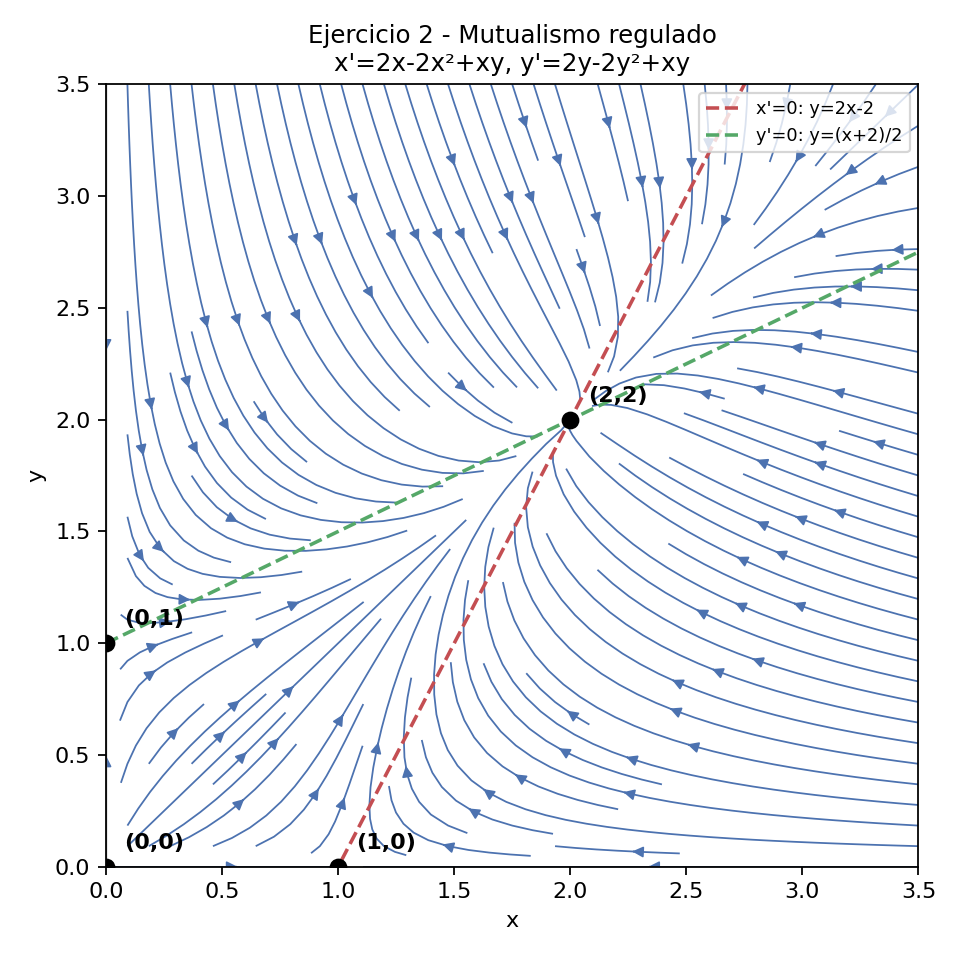
\includegraphics[width=0.72\textwidth]{figs/ejercicio2_mutualismo_regulado.png}
  \caption{Retrato fase del sistema mutualista regulado. Las isoclinas $y=2x-2$ (rojo) e
           $y=(x+2)/2$ (verde) se cortan en $(2,2)$, nodo sumidero estable. Toda trayectoria
           interior converge a ese punto.}
\end{figure}

\bigskip
\noindent\textbf{g) Conclusiones biológicas y comparación con Ejercicio~1.}

\begin{table}[H]
\centering
\begin{tabular}{ll}
\toprule
Condición inicial & Comportamiento a largo plazo \\
\midrule
$x_0=0,\;y_0=0$ & Extinción total (inestable) \\
$x_0>0,\;y_0=0$ & $\to(1,0)$: sobrevive solo $x$ en su capacidad de carga individual \\
$x_0=0,\;y_0>0$ & $\to(0,1)$: sobrevive solo $y$ \\
$x_0>0,\;y_0>0$ & $\to(2,2)$: \textbf{coexistencia estable y acotada} \\
\bottomrule
\end{tabular}
\end{table}

\begin{itemize}
  \item Punto de coexistencia: en el Ejercicio 1 es $(-2,-2)$, fuera del dominio; en el Ejercicio 2 es $(2,2)$, dentro del dominio y estable.
  \item Comportamiento interior: en el Ejercicio 1 hay crecimiento no acotado; en el Ejercicio 2 hay convergencia a $(2,2)$.
  \item Naturaleza: el Ejercicio 1 describe un mutualismo no saturado; el Ejercicio 2 describe un mutualismo regulado y biológicamente viable.
\end{itemize}

Basta con aumentar la autorregulación y reducir el coeficiente de cooperación para que el mutualismo pase de ``explosivo'' a regulado. El mutualismo es biológicamente viable solo si está saturado por la competencia interna.

\bigskip
\noindent\rule{\textwidth}{0.3pt}
\bigskip

% ============================================================
\noindent\textbf{Ejercicio 3.} Considérese el siguiente sistema de ecuaciones diferenciales
\[
  x' = 2x - x^2 - 2xy, \qquad y' = 2y - y^2 - 2xy.
\]

\noindent\textbf{a) Interpretación biológica.}

Factorizando:
\[
  x' = x(2-x-2y), \qquad y' = y(2-y-2x).
\]
\[
  \frac{x'}{x} = 2-x-2y, \qquad \frac{y'}{y} = 2-y-2x.
\]

Los términos $-2xy$ en ambas ecuaciones tienen signo negativo:
\[
  \frac{\partial}{\partial y}\!\left(\frac{x'}{x}\right)=-2<0,
  \qquad
  \frac{\partial}{\partial x}\!\left(\frac{y'}{y}\right)=-2<0.
\]
La presencia de la otra especie \emph{reduce} la tasa de crecimiento per cápita de ambas.
El sistema modela \textbf{competencia interespecífica} (tipo Lotka--Volterra de competencia).

\bigskip
\noindent\textbf{b) Puntos de equilibrio.}

De $x'=0$: $x=0$ o $x = 2-2y$.
De $y'=0$: $y=0$ o $y = 2-2x$.

\begin{itemize}
  \item $x=0,\,y=0 \;\to\; (0,0)$.
  \item $y=0$: $x(2-x)=0 \Rightarrow x=2 \;\to\; (2,0)$.
  \item $x=0$: $y(2-y)=0 \Rightarrow y=2 \;\to\; (0,2)$.
  \item $x=2-2y$ y $y=2-2x$: sustituyendo,
    $x = 2-2(2-2x) = -2+4x \Rightarrow -3x=-2 \Rightarrow x=\tfrac{2}{3},\;y=\tfrac{2}{3}$.
\end{itemize}

\[
  \boxed{(0,0),\quad (2,0),\quad (0,2),\quad \left(\tfrac{2}{3},\tfrac{2}{3}\right).}
\]

Los cuatro son biológicamente válidos.

\bigskip
\noindent\textbf{c) Linealización.}

\[
  DF(x,y) = \begin{pmatrix} 2-2x-2y & -2x \\ -2y & 2-2y-2x \end{pmatrix}.
\]

\begin{table}[H]
\centering
\begin{tabular}{lccc}
\toprule
Equilibrio & Jacobiana & Valores propios & Clasificación \\
\midrule
$(0,0)$ & $\begin{pmatrix}2&0\\0&2\end{pmatrix}$ & $2,\;2$ & Nodo fuente (inestable) \\[8pt]
$(2,0)$ & $\begin{pmatrix}-2&-4\\0&-2\end{pmatrix}$ & $-2,\;-2$ & Nodo estable (impropio) \\[8pt]
$(0,2)$ & $\begin{pmatrix}-2&0\\-4&-2\end{pmatrix}$ & $-2,\;-2$ & Nodo estable (impropio) \\[8pt]
$\left(\frac{2}{3},\frac{2}{3}\right)$ &
  $\begin{pmatrix}-2/3&-4/3\\-4/3&-2/3\end{pmatrix}$ & $\frac{2}{3},\;-2$ & \textbf{Punto silla} \\
\bottomrule
\end{tabular}
\end{table}

Para $\left(\tfrac23,\tfrac23\right)$: det $=\tfrac49-\tfrac{16}{9}=-\tfrac43<0$ (signo negativo
del determinante implica silla directamente). Verificando con el polinomio: $3\lambda^2+4\lambda-4=0$,
\[
  \lambda = \frac{-4\pm\sqrt{16+48}}{6} = \frac{-4\pm 8}{6}
  \;\Rightarrow\; \lambda_1=\tfrac{2}{3},\;\lambda_2=-2.
\]

El único equilibrio de coexistencia $\left(\tfrac23,\tfrac23\right)$ es \textbf{inestable (silla)}.

\bigskip
\noindent\textbf{d) Isoclinas nulas, separatriz y signos por región.}

Isoclinas no triviales: $L_1:\,x+2y=2$ (isoclina de $x$), $\;L_2:\,2x+y=2$ (isoclina de $y$).
Se intersectan en $\left(\tfrac23,\tfrac23\right)$. Los vectores propios de la silla determinan la
separatriz: $\lambda=-2$ tiene vector propio $(1,1)$, por lo que la \textbf{variedad estable es la diagonal $y=x$}.

\begin{table}[H]
\centering
\begin{tabular}{lccc}
\toprule
Punto de prueba & $x+2y$ vs $2$ & $2x+y$ vs $2$ & $(x',\;y')$ \\
\midrule
$(0.3,\,0.3)$ & $<2$ & $<2$ & $(+,+)$ \\
$(2,\,2)$ & $>2$ & $>2$ & $(-,-)$ \\
$(0.2,\,1.5)$ & $>2$ & $<2$ & $(-,+)$ \\
$(1.5,\,0.2)$ & $<2$ & $>2$ & $(+,-)$ \\
\bottomrule
\end{tabular}
\end{table}

\bigskip
\noindent\textbf{e) Bosquejo del retrato fase.}

\begin{figure}[H]
  \centering
  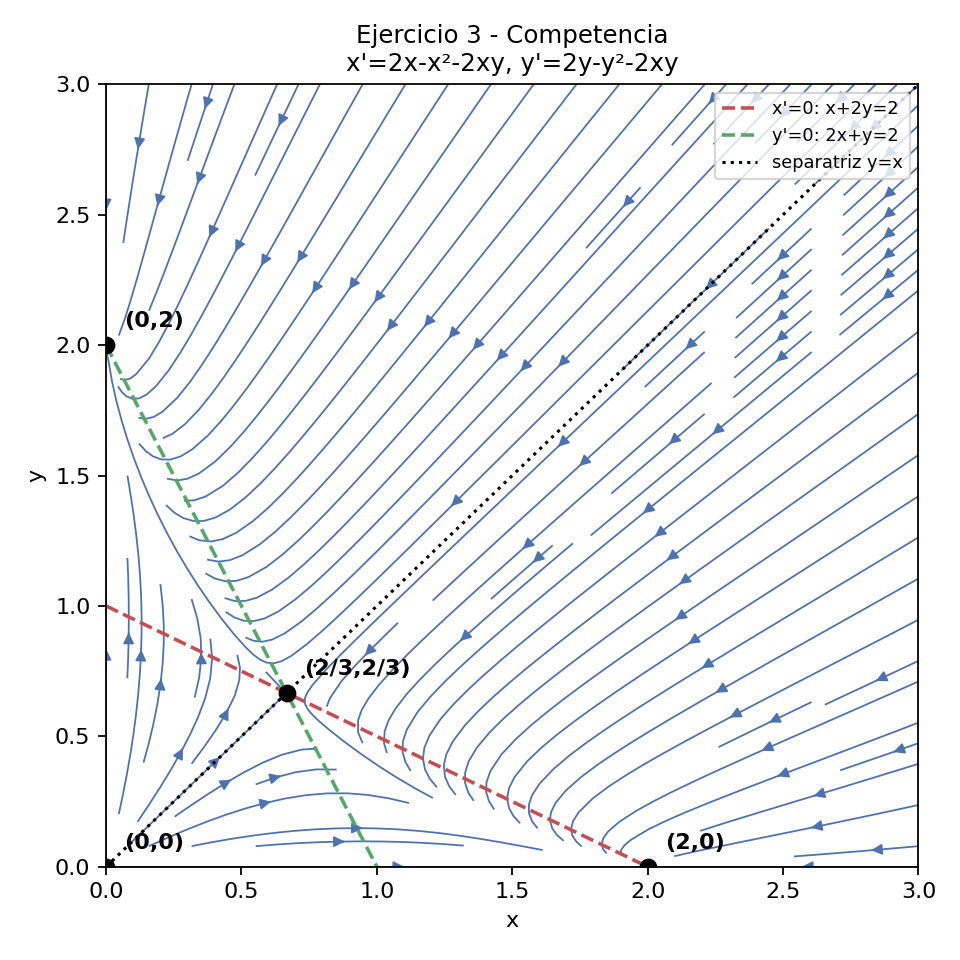
\includegraphics[width=0.72\textwidth]{figs/ejercicio3_competencia.png}
  \caption{Retrato fase del sistema de competencia. Las isoclinas $x+2y=2$ (rojo) y
           $2x+y=2$ (verde) se cortan en el punto silla $(\frac{2}{3},\frac{2}{3})$.
           La diagonal $y=x$ (punteada) actúa como separatriz entre las cuencas de atracción
           de $(2,0)$ y $(0,2)$.}
\end{figure}

\bigskip
\noindent\textbf{f) Conclusiones biológicas.}

\begin{table}[H]
\centering
\begin{tabular}{ll}
\toprule
Condición inicial & Comportamiento a largo plazo \\
\midrule
$x_0=0,\;y_0=0$ & Extinción total (inestable) \\
$x_0>0,\;y_0=0$ & $\to(2,0)$: solo sobrevive $x$ \\
$x_0=0,\;y_0>0$ & $\to(0,2)$: solo sobrevive $y$ \\
$x_0>y_0>0$ & $\to(2,0)$: $x$ excluye a $y$ \\
$y_0>x_0>0$ & $\to(0,2)$: $y$ excluye a $x$ \\
$x_0=y_0>0$ & $\to\left(\frac{2}{3},\frac{2}{3}\right)$: coexistencia, pero inestable \\
\bottomrule
\end{tabular}
\end{table}

El resultado ilustra el \textbf{Principio de Exclusión Competitiva}: aunque existe un punto de coexistencia, es una silla y no es robusto ante perturbaciones. En la práctica, la especie que parte con ventaja relativa (mayor densidad inicial) desplaza a la otra.

\bigskip
\noindent\rule{\textwidth}{0.3pt}
\bigskip

% ============================================================
\section*{Problemas de cálculo de isoclinas nulas}

% ─────────────────────────────────────────
\noindent\textbf{Problema 1.} Sistema
\[
  x' = x+y-4, \qquad y' = x-2y-1.
\]

\textbf{Isoclinas:}
\[
  x'=0 \;\Rightarrow\; y=4-x, \qquad y'=0 \;\Rightarrow\; y=\frac{x-1}{2}.
\]

\textbf{Equilibrio:} igualando $4-x=\tfrac{x-1}{2}$:
\[
  8-2x = x-1 \;\Rightarrow\; 9=3x \;\Rightarrow\; x=3,\;y=1.
  \qquad \boxed{(3,1).}
\]

\textbf{Clasificación:} $J=\begin{pmatrix}1&1\\1&-2\end{pmatrix}$,
traza $=-1$, det $=-3$, $\lambda^2+\lambda-3=0$,
$\lambda=\tfrac{-1\pm\sqrt{13}}{2}\approx 1.30,\,-2.30$. Signos opuestos: \textbf{punto silla}.

\textbf{Signos por región} ($A=x+y-4$, $B=x-2y-1$):

\begin{table}[H]
\centering
\begin{tabular}{lccc}
\toprule
Punto de prueba & $A$ & $B$ & $(x',\;y')$ \\
\midrule
$(5,\,0)$   & $1>0$  & $4>0$  & $(+,+)$ \\
$(3,\,5)$   & $4>0$  & $-8<0$ & $(+,-)$ \\
$(3,\,-3)$  & $-4<0$ & $8>0$  & $(-,+)$ \\
$(0,\,0)$   & $-4<0$ & $-1<0$ & $(-,-)$ \\
\bottomrule
\end{tabular}
\end{table}

\begin{figure}[H]
  \centering
  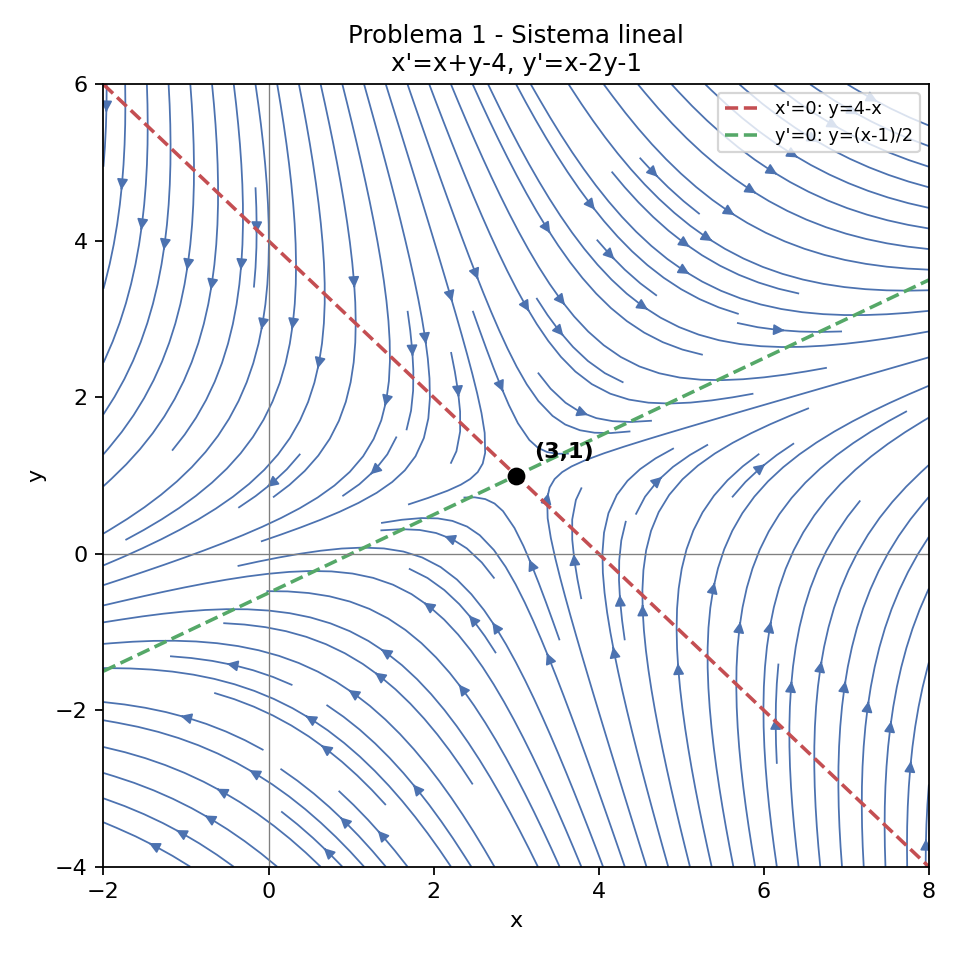
\includegraphics[width=0.62\textwidth]{figs/problema1_lineal.png}
  \caption{Retrato fase del Problema~1. Las dos rectas isoclinas se cruzan en el punto
           silla $(3,1)$.}
\end{figure}

\bigskip
% ─────────────────────────────────────────
\noindent\textbf{Problema 2.} Sistema
\[
  x' = x(1-y), \qquad y' = y(x-2).
\]

\textbf{Isoclinas:} $x'=0 \Rightarrow x=0$ o $y=1$. $\quad y'=0 \Rightarrow y=0$ o $x=2$.

\textbf{Equilibrios:}
\[
  \boxed{(0,0),\quad (2,1).}
\]

\textbf{Jacobiana:} $J=\begin{pmatrix}1-y&-x\\y&x-2\end{pmatrix}$.

\begin{itemize}
  \item $(0,0)$: $\lambda=1,-2$ $\to$ \textbf{silla}.
  \item $(2,1)$: traza $=0$, det $=2$, $\lambda=\pm i\sqrt{2}$ $\to$ \textbf{centro} (linealización, no hiperbólico).
\end{itemize}

\textbf{Signos por región} (primer cuadrante, dividido por $x=2$ e $y=1$):

\begin{table}[H]
\centering
\begin{tabular}{lcc}
\toprule
Región & $x'$ & $y'$ \\
\midrule
$0<x<2,\;0<y<1$ & $+$ & $-$ \\
$x>2,\;0<y<1$ & $+$ & $+$ \\
$0<x<2,\;y>1$ & $-$ & $-$ \\
$x>2,\;y>1$ & $-$ & $+$ \\
\bottomrule
\end{tabular}
\end{table}

El patrón de signos gira en sentido antihorario alrededor de $(2,1)$: comportamiento típico de órbitas cerradas (ciclos depredador--presa).

\begin{figure}[H]
  \centering
  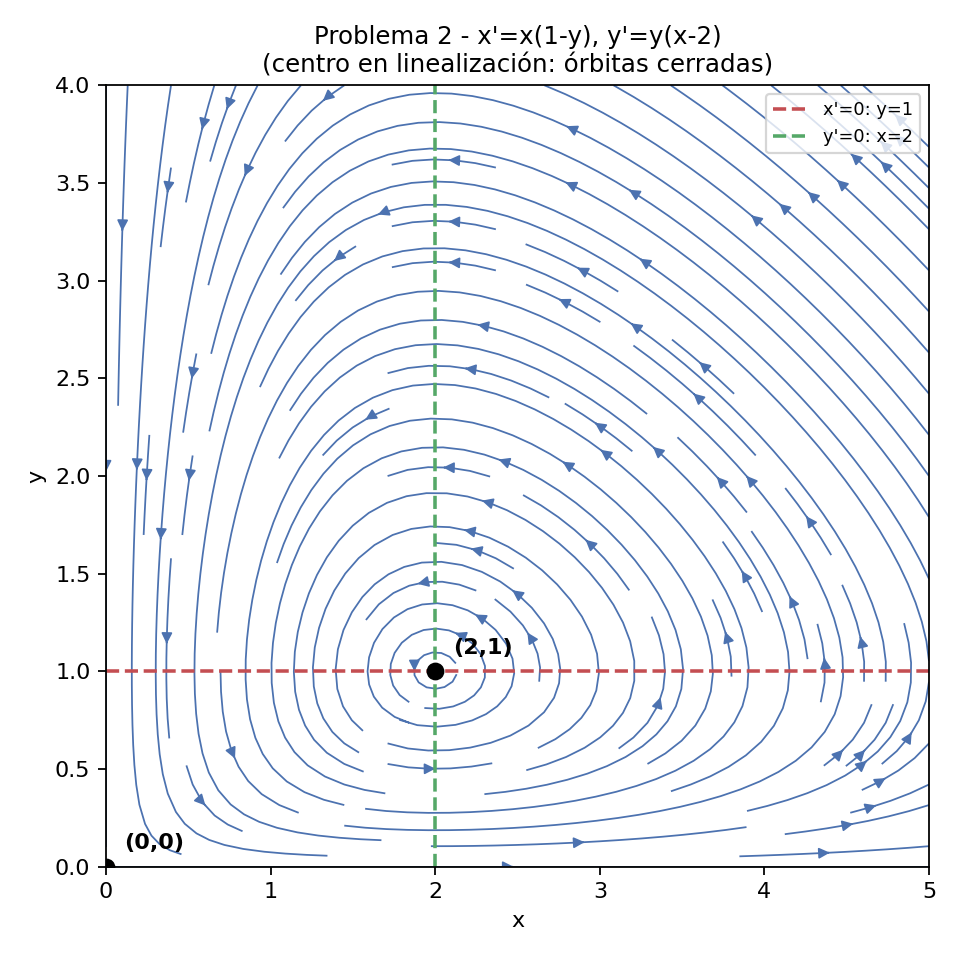
\includegraphics[width=0.62\textwidth]{figs/problema2_depredador_presa.png}
  \caption{Retrato fase del Problema~2. Las isoclinas $y=1$ (rojo) y $x=2$ (verde) se
           cortan en el centro $(2,1)$; las trayectorias describen órbitas cerradas en torno a él.}
\end{figure}

\bigskip
% ─────────────────────────────────────────
\noindent\textbf{Problema 3.} Sistema
\[
  x' = -y+x^2, \qquad y' = x+y^2.
\]

\textbf{Isoclinas:} $x'=0 \Rightarrow y=x^2$ (parábola). $\quad y'=0 \Rightarrow x=-y^2$ (parábola acostada).

\textbf{Equilibrios:} sustituyendo $y=x^2$ en $x=-y^2=-x^4$:
\[
  x+x^4=0 \;\Rightarrow\; x(1+x^3)=0 \;\Rightarrow\; x=0 \;\text{ ó }\; x=-1.
\]
\[
  \boxed{(0,0),\quad (-1,1).}
\]
Verificación de $(-1,1)$: $x=-y^2=-1$. $\checkmark$

\textbf{Jacobiana:} $J=\begin{pmatrix}2x&-1\\1&2y\end{pmatrix}$.
\begin{itemize}
  \item $(0,0)$: $\lambda=\pm i$ $\to$ \textbf{centro} (no hiperbólico, H--G no aplica).
  \item $(-1,1)$: traza $=0$, det $=-4+1=-3$, $\lambda=\pm\sqrt{3}$ $\to$ \textbf{silla}.
\end{itemize}

\textbf{Signos por región} (puntos de prueba):

\begin{table}[H]
\centering
\begin{tabular}{lccc}
\toprule
Punto & $x'=-y+x^2$ & $y'=x+y^2$ & $(x',\;y')$ \\
\midrule
$(1,\,0)$  & $1>0$  & $1>0$  & $(+,+)$ \\
$(0,\,1)$  & $-1<0$ & $1>0$  & $(-,+)$ \\
$(-2,\,0)$ & $4>0$  & $-2<0$ & $(+,-)$ \\
$(0,\,-1)$ & $1>0$  & $1>0$  & $(+,+)$ \\
\bottomrule
\end{tabular}
\end{table}

\begin{figure}[H]
  \centering
  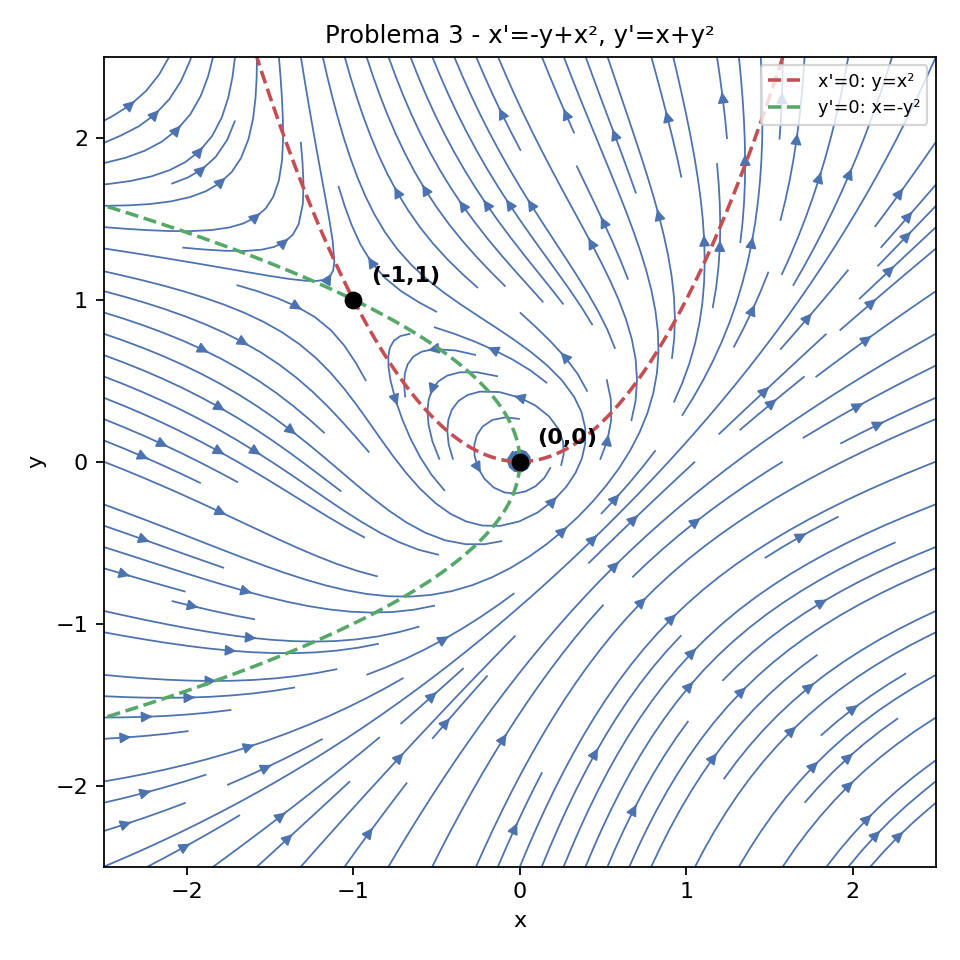
\includegraphics[width=0.62\textwidth]{figs/problema3_parabolas.png}
  \caption{Retrato fase del Problema~3. La parábola $y=x^2$ (rojo, isoclina de $x$) y la
           parábola acostada $x=-y^2$ (verde, isoclina de $y$) se cortan en $(0,0)$ y $(-1,1)$.}
\end{figure}

\bigskip
% ─────────────────────────────────────────
\noindent\textbf{Problema 4.} Sistema
\[
  x' = x(1-x-y), \qquad y' = y(2-x).
\]

\textbf{Isoclinas:} $x'=0 \Rightarrow x=0$ o $x+y=1$. $\quad y'=0 \Rightarrow y=0$ o $x=2$.

\textbf{Equilibrios:}
\[
  \boxed{(0,0),\quad (1,0).}
\]
La intersección $x+y=1$ con $x=2$ da $y=-1$: fuera del dominio biológico.

\textbf{Discusión de intersecciones:} la recta $x+y=1$ (capacidad de carga de $x$) corta a
$x=2$ en $y=-1$, fuera del primer cuadrante. Mientras $x\leq1$, siempre $x<2$, por lo que
$y'=y(2-x)>0$ para todo $y>0$: en el dominio biológico, $y$ crece sin cota.

\textbf{Clasificación:}
\begin{itemize}
  \item $(0,0)$: $\lambda=1,2$ $\to$ nodo fuente inestable.
  \item $(1,0)$: $J=\begin{pmatrix}-1&-1\\0&1\end{pmatrix}$, $\lambda=-1,1$ $\to$ \textbf{silla}.
\end{itemize}

\textbf{Signos:}

\begin{table}[H]
\centering
\begin{tabular}{lccc}
\toprule
Punto & $x+y$ vs $1$ & $x$ vs $2$ & $(x',\;y')$ \\
\midrule
$(0.3,\,0.3)$ & $<1$ & $<2$ & $(+,+)$ \\
$(0.7,\,0.7)$ & $>1$ & $<2$ & $(-,+)$ \\
$(3,\,0.5)$ & $>1$ & $>2$ & $(-,-)$ \\
\bottomrule
\end{tabular}
\end{table}

\begin{figure}[H]
  \centering
  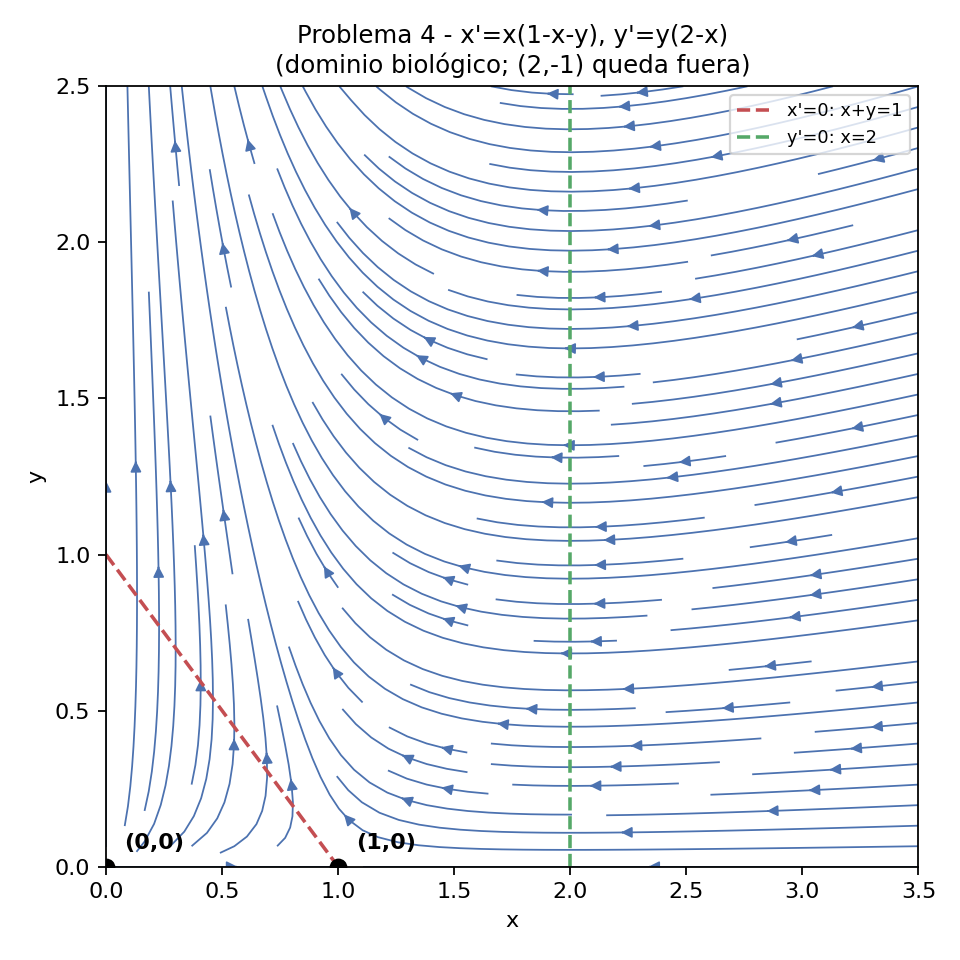
\includegraphics[width=0.62\textwidth]{figs/problema4_biologico.png}
  \caption{Retrato fase del Problema~4. La recta $x+y=1$ (rojo) y la recta $x=2$ (verde)
           no se intersectan en el primer cuadrante: la nullclina $x=2$ queda inalcanzable
           para las trayectorias biológicas.}
\end{figure}

\bigskip
% ─────────────────────────────────────────
\noindent\textbf{Problema 5.} Sistema
\[
  x' = -y+x(x^2+y^2), \qquad y' = x+y(x^2+y^2).
\]

\textbf{Equilibrios:} solo $(0,0)$ (para $r\neq0$ se llega a $\tan^2\theta=-1$, sin solución real).

\textbf{Jacobiana en el origen:} $J(0,0)=\begin{pmatrix}0&-1\\1&0\end{pmatrix}$,
$\lambda=\pm i$ (centro, no hiperbólico).

\textbf{Análisis exacto en coordenadas polares} ($x=r\cos\theta$, $y=r\sin\theta$):
\[
  r' = \frac{xx'+yy'}{r} = \frac{x(-y+xr^2)+y(x+yr^2)}{r} = \frac{r^2(x^2+y^2)}{r} = r^3.
\]
\[
  \theta' = 1.
\]
Como $r'=r^3>0$ para $r>0$, el radio crece siempre: el origen es en realidad un
\textbf{foco inestable}. Resolviendo $dr/dt=r^3$:
\[
  r(t) = \frac{1}{\sqrt{r_0^{-2}-2t}}, \qquad
  \text{explosión en tiempo finito } t^* = \frac{1}{2r_0^2}.
\]

\begin{figure}[H]
  \centering
  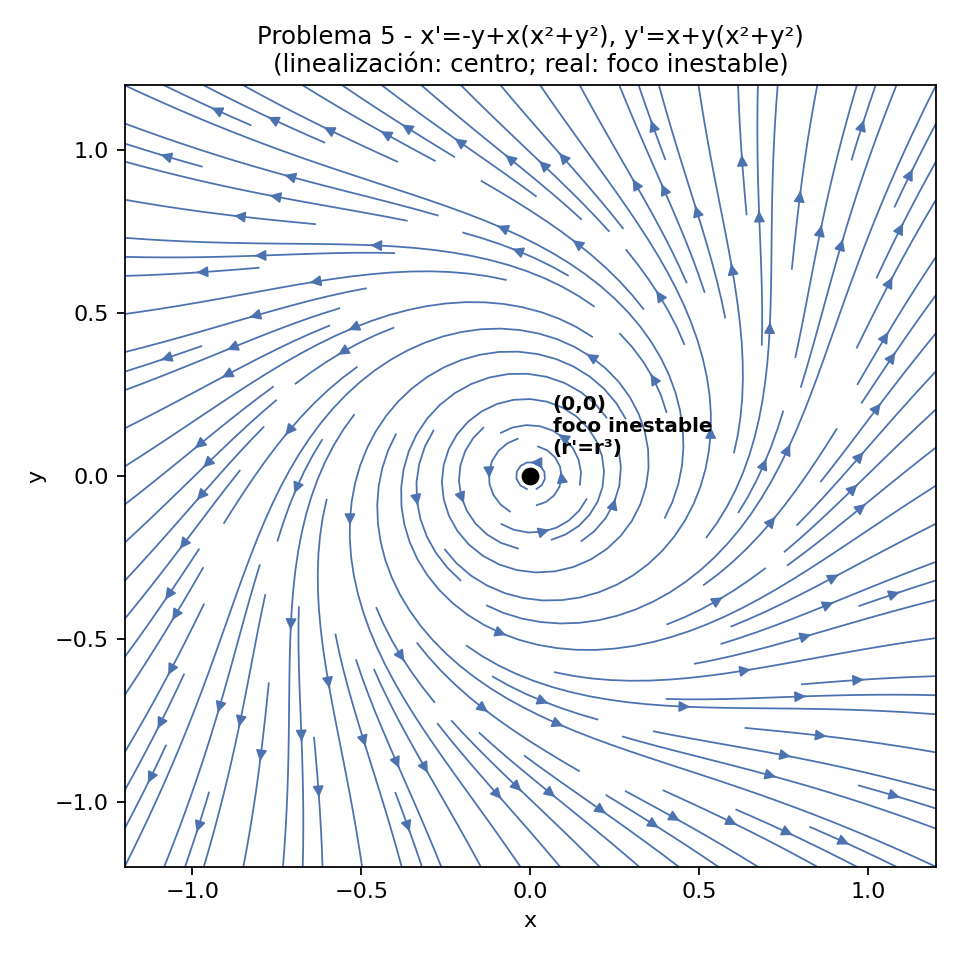
\includegraphics[width=0.62\textwidth]{figs/problema5_foco_inestable.png}
  \caption{Retrato fase del Problema~5. Aunque la linealización predice un centro, el análisis
           en polares revela un foco inestable: las trayectorias espiralan hacia afuera y escapan
           en tiempo finito.}
\end{figure}

\bigskip
% ─────────────────────────────────────────
\noindent\textbf{Problema 6.} Sistema de Lotka--Volterra:
\[
  x' = \alpha x - \beta xy, \qquad y' = -\delta y + \gamma xy.
\]

\textbf{Isoclinas:} $x'=0 \Rightarrow x=0$ o $y=\alpha/\beta$. $\quad y'=0 \Rightarrow y=0$ o $x=\delta/\gamma$.

\textbf{Equilibrios:}
\[
  \boxed{(0,0),\qquad \left(\frac{\delta}{\gamma},\,\frac{\alpha}{\beta}\right).}
\]

\textbf{Jacobiana:} $J=\begin{pmatrix}\alpha-\beta y&-\beta x\\\gamma y&-\delta+\gamma x\end{pmatrix}$.

\begin{itemize}
  \item $(0,0)$: $\lambda=\alpha,-\delta$ (signos opuestos) $\to$ \textbf{silla}.
  \item $\left(\tfrac\delta\gamma,\tfrac\alpha\beta\right)$: traza $=0$, det $=\alpha\delta>0$,
    $\lambda=\pm i\sqrt{\alpha\delta}$ $\to$ \textbf{centro} (robusto por la cantidad conservada
    $H=\gamma x-\delta\ln x+\beta y-\alpha\ln y$).
\end{itemize}

\textbf{Signos} (primer cuadrante, dividido por $x=\delta/\gamma$ e $y=\alpha/\beta$):

\begin{table}[H]
\centering
\begin{tabular}{lcc}
\toprule
Región & $x'$ & $y'$ \\
\midrule
$x<\delta/\gamma,\;y<\alpha/\beta$ & $+$ & $-$ \\
$x>\delta/\gamma,\;y<\alpha/\beta$ & $+$ & $+$ \\
$x>\delta/\gamma,\;y>\alpha/\beta$ & $-$ & $+$ \\
$x<\delta/\gamma,\;y>\alpha/\beta$ & $-$ & $-$ \\
\bottomrule
\end{tabular}
\end{table}

Rotación antihoraria: las trayectorias son ciclos cerrados (oscilaciones periódicas depredador--presa).

\begin{figure}[H]
  \centering
  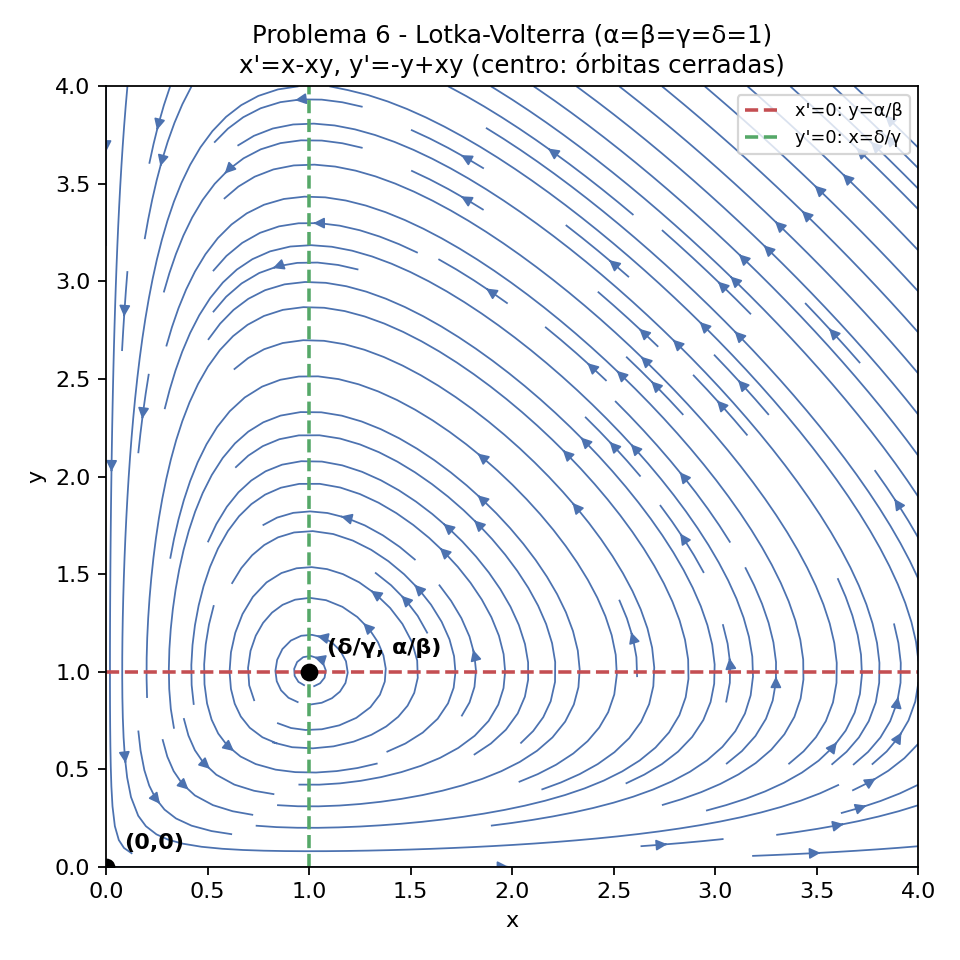
\includegraphics[width=0.62\textwidth]{figs/problema6_lotka_volterra.png}
  \caption{Retrato fase del Problema~6 con $\alpha=\beta=\gamma=\delta=1$. El equilibrio interior
           $(1,1)$ es un centro rodeado por órbitas cerradas; el origen es silla.}
\end{figure}

\bigskip
\noindent\rule{\textwidth}{0.3pt}
\bigskip

% ============================================================
\noindent\textbf{Ejercicio 4.} Análisis de ciclos límite.

\textbf{Recordatorio:} si existe $B(x,y)\in C^1(D)$ tal que
$\tfrac{\partial(Bf)}{\partial x}+\tfrac{\partial(Bg)}{\partial y}$
tiene signo constante en una región simplemente conexa $D$, entonces el sistema
$x'=f,\;y'=g$ \textbf{no tiene ciclos límite} en $D$.

\bigskip
\noindent\textbf{(a)} $x'=y$, $\;y'=-ax-by+\alpha x^2+\beta y^2$.

Tomamos $B(x,y)=e^{-2\beta x}$.

\[
  Bf = e^{-2\beta x}\,y, \qquad
  \frac{\partial(Bf)}{\partial x} = -2\beta\,e^{-2\beta x}\,y.
\]
\[
  Bg = e^{-2\beta x}\!\left(-ax-by+\alpha x^2+\beta y^2\right), \qquad
  \frac{\partial(Bg)}{\partial y} = e^{-2\beta x}(-b+2\beta y).
\]

Sumando:
\[
  \frac{\partial(Bf)}{\partial x}+\frac{\partial(Bg)}{\partial y}
  = e^{-2\beta x}\!\left[-2\beta y + (-b+2\beta y)\right]
  = e^{-2\beta x}(\underbrace{-2\beta y+2\beta y}_{0}-b)
  = \boxed{-b\,e^{-2\beta x}.}
\]

Como $e^{-2\beta x}>0$ para todo $x\in\mathbb{R}$ y $b$ tiene signo fijo, la expresión tiene
signo constante en todo $\mathbb{R}^2$. Por el argumento anterior, el sistema
\textbf{no admite ciclos límite}.

\bigskip
\noindent\textbf{(b)} $\displaystyle x'=\frac{y}{1+x^2}$, $\;\displaystyle y'=\frac{-x+y(1+x^2+y^4)}{1+x^2}$.

Tomamos $B(x,y)=1+x^2$.

\[
  Bf = (1+x^2)\cdot\frac{y}{1+x^2} = y, \qquad
  \frac{\partial(Bf)}{\partial x} = 0.
\]
\[
  Bg = (1+x^2)\cdot\frac{-x+y(1+x^2+y^4)}{1+x^2}
     = -x+y+x^2y+y^5.
\]
\[
  \frac{\partial(Bg)}{\partial y} = 1+x^2+5y^4.
\]

Sumando:
\[
  \frac{\partial(Bf)}{\partial x}+\frac{\partial(Bg)}{\partial y}
  = \boxed{1+x^2+5y^4.}
\]

Esta expresión satisface $1+x^2+5y^4 \geq 1>0$ para todo $(x,y)\in\mathbb{R}^2$. Por el argumento anterior, el sistema \textbf{no presenta ciclos límite} en $\mathbb{R}^2$.

\bigskip
\noindent\rule{\textwidth}{0.3pt}
\bigskip

% ============================================================
\section*{Problemas: Teorema de Hartman--Grobman}

\noindent\textbf{Recordatorio.} Si el equilibrio $X_0$ de $\dot X=F(X)$ es hiperbólico
(ningún valor propio de $DF(X_0)$ tiene parte real nula), entonces el sistema no lineal es
localmente homeomorfo a su linealización $\dot Y=DF(X_0)Y$ en un entorno de $X_0$.

\bigskip
% ─────────────────────────────────────────
\noindent\textbf{Problema 1 (Plano). El punto de silla clásico.}
\[
  \dot x = x+y^2, \qquad \dot y = -y+x^2.
\]

\textbf{Equilibrio en el origen:}
$f(0,0)=0+0=0$, $g(0,0)=0+0=0$. $\checkmark$

\textbf{Jacobiana:}
\[
  DF(x,y)=\begin{pmatrix}1&2y\\2x&-1\end{pmatrix},
  \qquad
  J(0,0)=\begin{pmatrix}1&0\\0&-1\end{pmatrix}.
\]

\textbf{Valores propios:} polinomio $(1-\lambda)(-1-\lambda)=\lambda^2-1=0 \Rightarrow$
\[
  \boxed{\lambda_1=1,\qquad \lambda_2=-1.}
\]

\textbf{Vectores propios:}
\begin{itemize}
  \item $\lambda_1=1$: $(J-I)v=0 \Rightarrow \begin{pmatrix}0&0\\0&-2\end{pmatrix}v=0
    \Rightarrow v_2=0$. Vector propio $v_1=(1,0)$ (dirección \textbf{inestable}, eje $x$).
  \item $\lambda_2=-1$: $(J+I)v=0 \Rightarrow \begin{pmatrix}2&0\\0&0\end{pmatrix}v=0
    \Rightarrow v_1=0$. Vector propio $v_2=(0,1)$ (dirección \textbf{estable}, eje $y$).
\end{itemize}

\textbf{Hartman--Grobman:} $\text{Re}(\lambda_1)=1\neq0$, $\text{Re}(\lambda_2)=-1\neq0$:
equilibrio \textbf{hiperbólico}. El sistema no lineal es localmente topológicamente equivalente
a la silla lineal. Existen variedades $W^s_{loc}$ (tangente al eje $y$) y $W^u_{loc}$
(tangente al eje $x$) para el sistema no lineal.

\bigskip
% ─────────────────────────────────────────
\noindent\textbf{Problema 2 (Plano). Un foco estable.}
\[
  \dot x = -x-2y+xy, \qquad \dot y = 2x-y-x^2.
\]

\textbf{Equilibrio en el origen:} $f(0,0)=0$, $g(0,0)=0$. $\checkmark$

\textbf{Jacobiana:}
\[
  DF(x,y)=\begin{pmatrix}-1+y&-2+x\\2-2x&-1\end{pmatrix},
  \qquad
  J(0,0)=\begin{pmatrix}-1&-2\\2&-1\end{pmatrix}.
\]

\textbf{Valores propios:} traza $=-2$, det $=1+4=5$,
\[
  \lambda^2+2\lambda+5=0 \;\Rightarrow\;
  \lambda = \frac{-2\pm\sqrt{4-20}}{2} = \frac{-2\pm4i}{2}.
  \qquad \boxed{\lambda_{1,2}=-1\pm2i.}
\]

\textbf{Hartman--Grobman:} $\text{Re}(\lambda)=-1\neq0$: equilibrio \textbf{hiperbólico}.
El sistema no lineal es localmente equivalente a un \textbf{foco estable}: las trayectorias
espiralan hacia el origen con tasa de decaimiento $e^{-t}$ y frecuencia $\omega=2$. A diferencia
del punto silla, \emph{todas} las trayectorias suficientemente cercanas convergen al origen.

\bigskip
% ─────────────────────────────────────────
\noindent\textbf{Problema 3 (Plano). Múltiples equilibrios y la frontera de la hiperbolicidad.}
\[
  \dot x = y, \qquad \dot y = x-x^3.
\]

\textbf{Equilibrios:} $y=0$ y $x-x^3=x(1-x)(1+x)=0$:
\[
  \boxed{(0,0),\quad (1,0),\quad (-1,0).}
\]

\textbf{Jacobiana:}
\[
  DF(x,y)=\begin{pmatrix}0&1\\1-3x^2&0\end{pmatrix}.
\]

\begin{table}[H]
\centering
\begin{tabular}{lccc}
\toprule
Equilibrio & Jacobiana & Valores propios & ¿Hiperbólico? \\
\midrule
$(0,0)$ & $\begin{pmatrix}0&1\\1&0\end{pmatrix}$ & $\lambda^2-1=0 \Rightarrow \pm1$ & \textbf{Sí} $\to$ silla \\[8pt]
$(1,0)$ & $\begin{pmatrix}0&1\\-2&0\end{pmatrix}$ & $\lambda^2+2=0 \Rightarrow \pm i\sqrt2$ & \textbf{No} (parte real $=0$) \\[8pt]
$(-1,0)$ & $\begin{pmatrix}0&1\\-2&0\end{pmatrix}$ & $\pm i\sqrt2$ & \textbf{No} (parte real $=0$) \\
\bottomrule
\end{tabular}
\end{table}

\textbf{Conclusión:}
\begin{itemize}
  \item \textbf{En $(0,0)$:} valores propios reales $\pm1$, parte real $\neq0$ $\Rightarrow$ hiperbólico.
    Hartman--Grobman \textbf{sí aplica}: el sistema no lineal es localmente equivalente a una silla.
  \item \textbf{En $(\pm1,0)$:} valores propios puramente imaginarios $\Rightarrow$ \textbf{no hiperbólico}.
  \item[] Hartman--Grobman \textbf{no aplica}: la linealización predice centro, pero el
    comportamiento real depende de términos de orden superior. En este caso, el comportamiento
    real confirma centros verdaderos, pero por la estructura del sistema, \emph{no} por el teorema.
\end{itemize}

\bigskip
% ─────────────────────────────────────────
\noindent\textbf{Problema 7 (Espacio $\mathbb{R}^3$). Silla-Foco en 3D.}
\[
  \dot x = -x-y+z^2, \qquad \dot y = x-y-xz, \qquad \dot z = 2z+xy.
\]

\textbf{Equilibrio en el origen:} $f(0,0,0)=0$, $g(0,0,0)=0$, $h(0,0,0)=0$. $\checkmark$

\textbf{Jacobiana:}
\[
  DF(x,y,z)=\begin{pmatrix}-1&-1&2z\\1-z&-1&-x\\y&x&2\end{pmatrix},
  \qquad
  J(0,0,0)=\begin{pmatrix}-1&-1&0\\1&-1&0\\0&0&2\end{pmatrix}.
\]

La estructura de bloques desacopla el eje $z$ del subespacio $(x,y)$.

\textbf{Bloque $(x,y)$:}
\[
  A=\begin{pmatrix}-1&-1\\1&-1\end{pmatrix},\quad
  \text{traza}=-2,\quad \det=2,\quad
  \lambda^2+2\lambda+2=0 \;\Rightarrow\; \lambda=-1\pm i.
\]

\textbf{Bloque $z$:} $\lambda_3=2$.

\[
  \boxed{\lambda_1=-1+i,\quad \lambda_2=-1-i,\quad \lambda_3=2.}
\]

\textbf{Hartman--Grobman:} $\text{Re}(\lambda_{1,2})=-1\neq0$, $\text{Re}(\lambda_3)=2\neq0$:
equilibrio \textbf{hiperbólico}. El sistema no lineal posee:
\begin{itemize}
  \item \textbf{Variedad estable local bidimensional} $W^s_{loc}$, tangente al plano $xy$
    (asociada a $\lambda_{1,2}=-1\pm i$): las trayectorias \textbf{espiralan hacia el origen}
    dentro de este plano.
  \item \textbf{Variedad inestable local unidimensional} $W^u_{loc}$, tangente al eje $z$
    (asociada a $\lambda_3=2$): las trayectorias \textbf{se alejan} del origen en esta dirección.
\end{itemize}
El origen es una \textbf{silla-foco}: atrae en espiral dentro de un plano pero repele a lo largo
de la dirección transversal $z$.

\bigskip
% ─────────────────────────────────────────
\noindent\textbf{Problema 8 (Espacio $\mathbb{R}^3$). Sistema de tres variables.}
\[
  \dot x = \sigma(y-x), \qquad \dot y = rx-y-xz, \qquad \dot z = xy-bz.
\]

\textbf{Linealización en el origen:}
\[
  DF(x,y,z)=\begin{pmatrix}-\sigma&\sigma&0\\r-z&-1&-x\\y&x&-b\end{pmatrix},
  \qquad
  \boxed{J(0,0,0)=\begin{pmatrix}-\sigma&\sigma&0\\r&-1&0\\0&0&-b\end{pmatrix}.}
\]

Estructura de bloques: eje $z$ desacoplado.

\textbf{Con $\sigma=10$, $b=8/3$, $r=28$:}

\textbf{Bloque $z$:} $\lambda_3=-b=-\tfrac83$.

\textbf{Bloque $(x,y)$:}
\[
  A=\begin{pmatrix}-10&10\\28&-1\end{pmatrix},\quad
  \text{traza}=-11,\quad \det=10(1-28)=-270.
\]
Como det $<0$, las raíces son reales con signos opuestos (sin resolver explícitamente).
Polinomio: $\lambda^2+11\lambda-270=0$:
\[
  \lambda=\frac{-11\pm\sqrt{121+1080}}{2}=\frac{-11\pm\sqrt{1201}}{2}
  \approx \frac{-11\pm34.66}{2}.
\]
\[
  \boxed{\lambda_1\approx11.83,\quad \lambda_2\approx-22.83,\quad \lambda_3\approx-2.67.}
\]

\textbf{Hartman--Grobman:} ningún valor propio tiene parte real nula $\Rightarrow$ el origen es
\textbf{hiperbólico}. Con dos valores propios negativos y uno positivo, es un \textbf{punto silla
generalizado} en $\mathbb{R}^3$:
\begin{itemize}
  \item \textbf{Variedad estable bidimensional} (asociada a $\lambda_2$ y $\lambda_3$).
  \item \textbf{Variedad inestable unidimensional} (asociada a $\lambda_1>0$).
\end{itemize}
Las trayectorias son expulsadas del origen, lo cual es consistente con la dirección inestable
obtenida por la linealización.

\bigskip
\noindent\rule{\textwidth}{0.5pt}

\begin{thebibliography}{1}
\bibitem{nagle}
R. Kent Nagle, Edward B. Saff y Arthur David Snider,
\textit{Fundamentals of Differential Equations and Boundary Value Problems},
7th ed., Pearson, Boston, 2018.
\end{thebibliography}

\end{document}
